\begin{longtable} { | c | p{12cm} | c | } 
\hline
	ID 	&	Issues	&		 Es. hours \\\hline
	34 	&	Implement choices in sequences	&	16 hours \\\hline
\caption{Issue ID 34}
\label{tab:spr3_choicesinsequences}
\end{longtable}

As choices was now able to add in sequences, we needed some way to display and editing choices. \note{INDSÆT BILLEDE AF DIALOGBOX MED CHOICE} The group focusing on `LivsHistorier' had a way to show and display choices, but we found that the theme of their dialog box did not fit well into `Sekvens'. We wanted to keep editing consistent within the application itself, so we chose to use the same \ct{ViewGroups} to have them completely similar. We created a fully customizable dialog box and created a new \ct{SequenceViewGroup} within it. The following listing shows how the code is written and how portrayed in figure \ref{fig:magicshit}

\begin{lstlisting}

   <HorizontalScrollView
        android:id="@+id/horizontalScrollView"
        android:layout_width="match_parent"
        android:layout_height="match_parent"
        android:layout_margin="0dp"
        android:overScrollMode="always"
        android:padding="0dp"
        android:fadeScrollbars="false">

        <FrameLayout
            android:layout_width="wrap_content"
            android:layout_height="match_parent">

            <dk.aau.cs.giraf.zebra.SequenceViewGroup
                android:id="@+id/sequenceViewGroup"
                android:layout_width="wrap_content"
                android:layout_height="wrap_content"
                android:layout_marginLeft="30dp"
                android:layout_marginRight="30dp"
                svg:horizontalSpacing="20dp"
                svg:itemHeight="@dimen/activity_main_picto_size"
                svg:itemWidth="@dimen/activity_main_picto_size"
                android:background="@layout/main_picto_container_bg"
                android:layout_gravity="center_vertical">
            </dk.aau.cs.giraf.zebra.SequenceViewGroup>
        </FrameLayout>
    </HorizontalScrollView>

\end{lstlisting}

This made the implementation really easy as all of the functionality we needed i choice already was implemented in \ct{SequenceViewGroup}. The features included adding pictograms to the choice, as well as arbitrary scrolling features and handling the views. The fully customizable dialogbox provided by the GUI-component group, made it easy to follow the overall theme. Figure \ref{fig:magicshit} is a representation of what creating a choice looks like.

\begin{figure} [H]
\centering
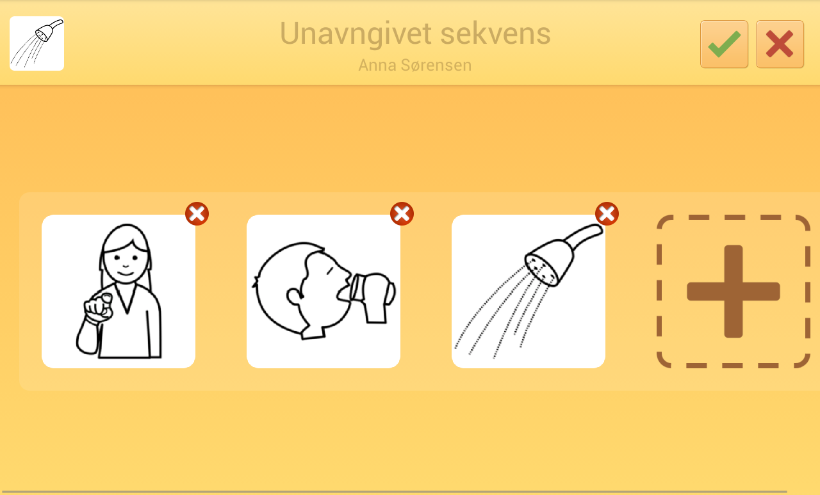
\includegraphics[width=14cm]{Pics/Sprint3/EditModeCropped}
\caption{THISISAPLACEHOLDER}
\label{fig:magicshit}
\end{figure}
